\documentclass{standalone}
\usepackage{tikz}
\usetikzlibrary{patterns, positioning}
\usepackage[sfdefault]{ClearSans} %% option 'sfdefault' activates Clear Sans as the default text font
\usepackage[T1]{fontenc}

\begin{document}
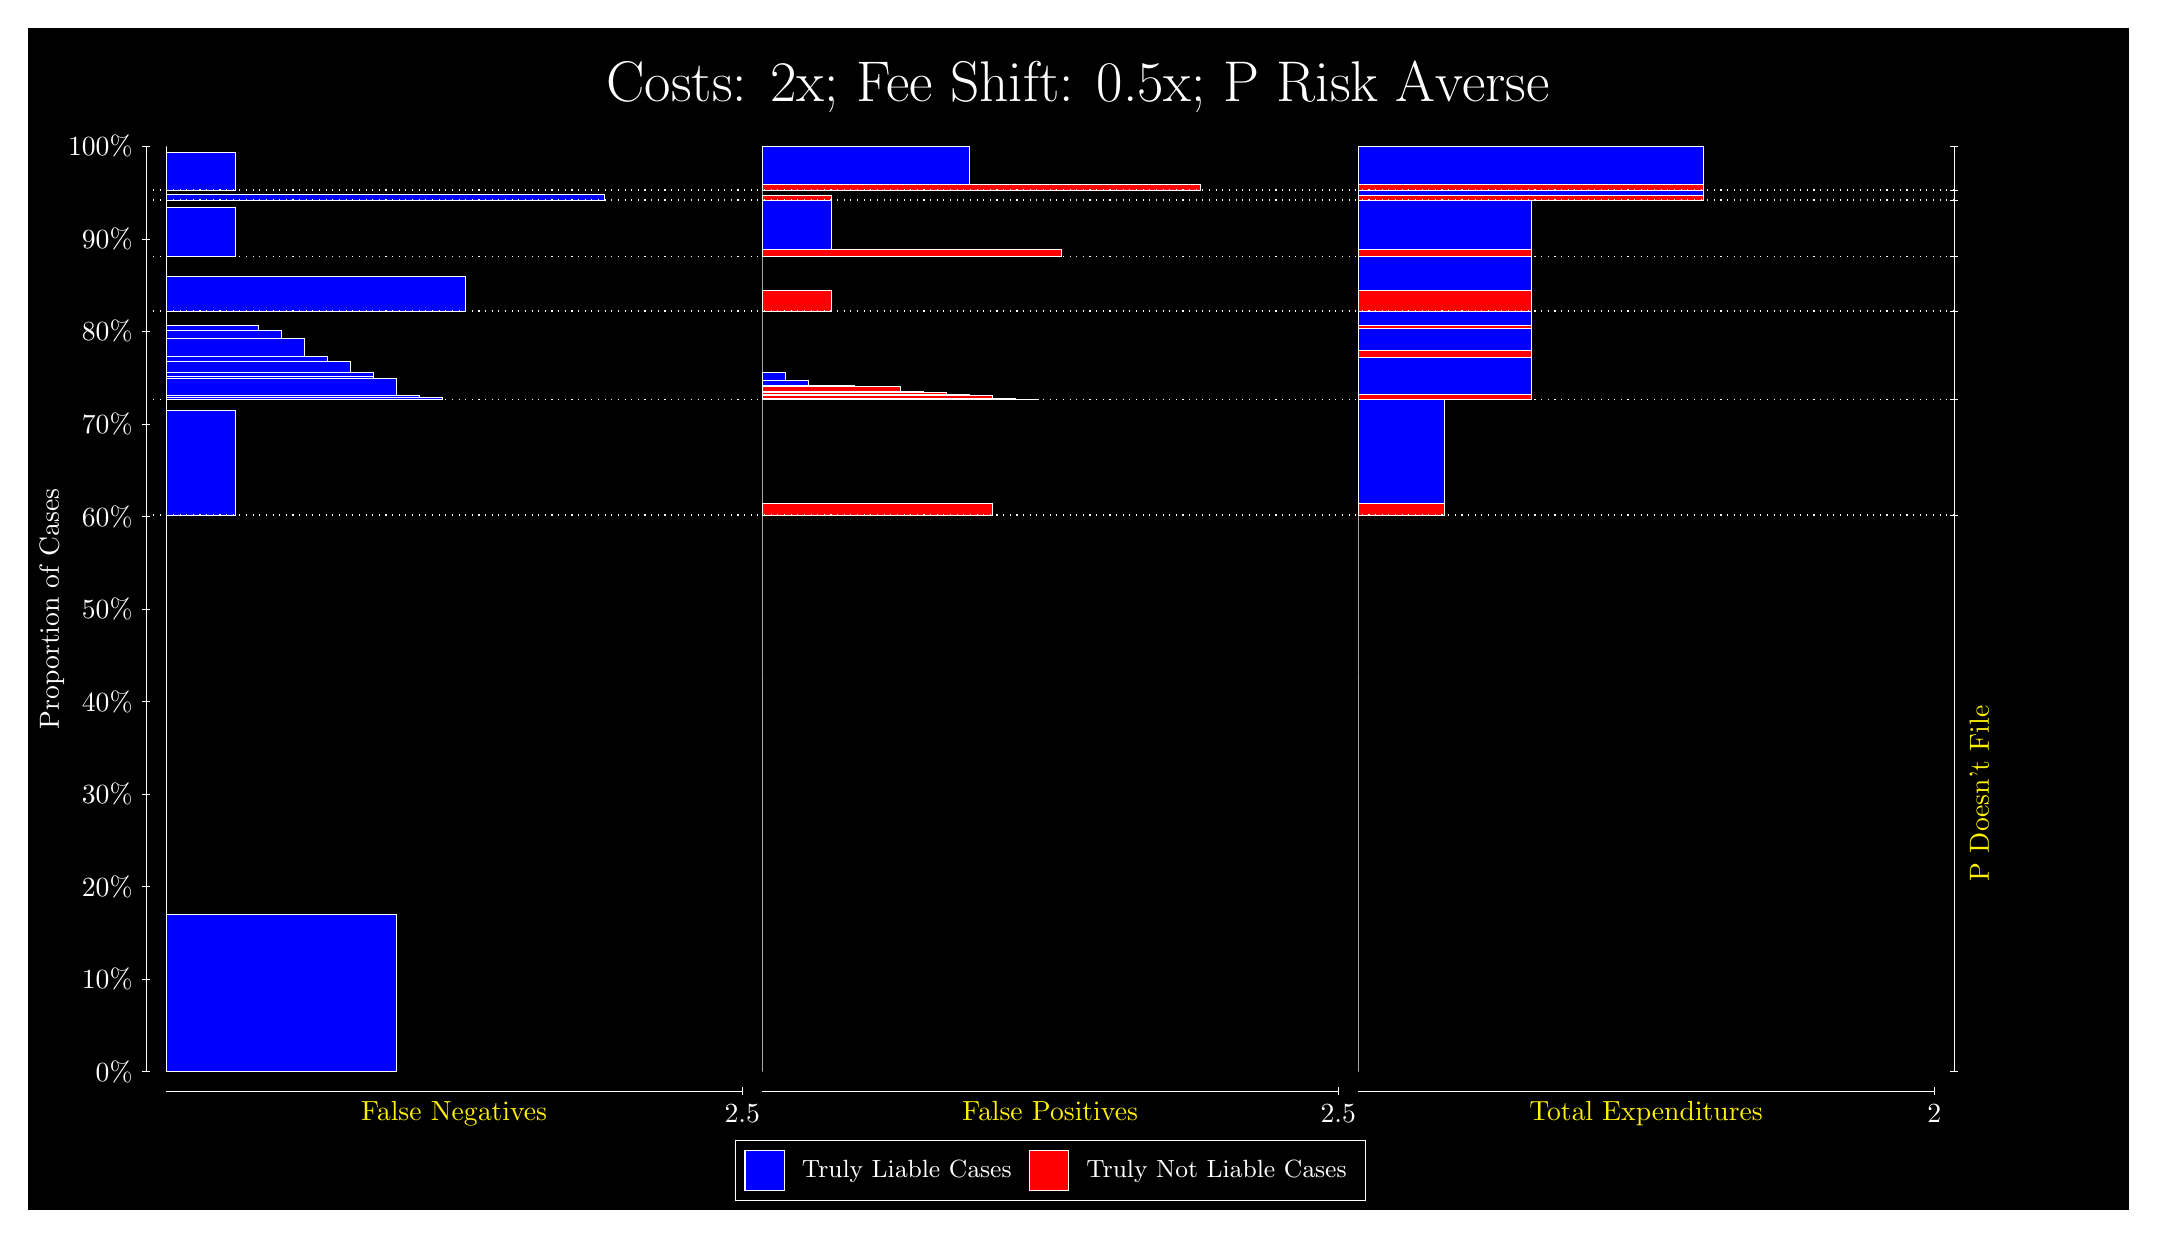
\begin{tikzpicture}
\draw[fill=black] (0,0) rectangle (26.667,15);
\draw[text=white] (0,13.5) rectangle (26.667,15) node[midway] {\huge Costs: 2x; Fee Shift: 0.5x; P Risk Averse};
\draw[white, very thin] (1.5,1.75) -- (1.5,13.5);
\node[rotate=90, text=white, anchor=center] at (0.3, 7.625) {Proportion of Cases};
\draw[white, very thin] (1.45,1.75) -- (1.55,1.75);
\node[text=white, anchor=east] at (1.45, 1.75) {0\%};
\draw[white, very thin] (1.45,2.925) -- (1.55,2.925);
\node[text=white, anchor=east] at (1.45, 2.925) {10\%};
\draw[white, very thin] (1.45,4.1) -- (1.55,4.1);
\node[text=white, anchor=east] at (1.45, 4.1) {20\%};
\draw[white, very thin] (1.45,5.275) -- (1.55,5.275);
\node[text=white, anchor=east] at (1.45, 5.275) {30\%};
\draw[white, very thin] (1.45,6.45) -- (1.55,6.45);
\node[text=white, anchor=east] at (1.45, 6.45) {40\%};
\draw[white, very thin] (1.45,7.625) -- (1.55,7.625);
\node[text=white, anchor=east] at (1.45, 7.625) {50\%};
\draw[white, very thin] (1.45,8.8) -- (1.55,8.8);
\node[text=white, anchor=east] at (1.45, 8.8) {60\%};
\draw[white, very thin] (1.45,9.975) -- (1.55,9.975);
\node[text=white, anchor=east] at (1.45, 9.975) {70\%};
\draw[white, very thin] (1.45,11.15) -- (1.55,11.15);
\node[text=white, anchor=east] at (1.45, 11.15) {80\%};
\draw[white, very thin] (1.45,12.325) -- (1.55,12.325);
\node[text=white, anchor=east] at (1.45, 12.325) {90\%};
\draw[white, very thin] (1.45,13.5) -- (1.55,13.5);
\node[text=white, anchor=east] at (1.45, 13.5) {100\%};

\draw[white, very thin] (24.457,1.75) -- (24.457,13.5);
\draw[white, very thin] (24.407,1.75) -- (24.507,1.75);
\node[anchor=west] at (24.407, 1.75) {};
\draw[white, very thin] (24.407,8.8182) -- (24.507,8.8182);
\node[anchor=west] at (24.407, 8.8182) {};
\draw[white, very thin] (24.407,10.286) -- (24.507,10.286);
\node[anchor=west] at (24.407, 10.286) {};
\draw[white, very thin] (24.407,11.409) -- (24.507,11.409);
\node[anchor=west] at (24.407, 11.409) {};
\draw[white, very thin] (24.407,12.105) -- (24.507,12.105);
\node[anchor=west] at (24.407, 12.105) {};
\draw[white, very thin] (24.407,12.818) -- (24.507,12.818);
\node[anchor=west] at (24.407, 12.818) {};
\draw[white, very thin] (24.407,12.945) -- (24.507,12.945);
\node[anchor=west] at (24.407, 12.945) {};
\draw[white, very thin] (24.407,13.5) -- (24.507,13.5);
\node[anchor=west] at (24.407, 13.5) {};

\draw[white, very thin, fill=blue] (1.75,1.75) rectangle (4.6775,3.749);
\draw[white, very thin, fill=red] (1.75,3.749) rectangle (1.75,8.8182);
\draw[white, very thin, fill=blue] (1.75,8.8182) rectangle (2.6283,10.144);
\draw[white, very thin, fill=red] (1.75,10.144) rectangle (1.75,10.286);
\draw[white, very thin, fill=blue] (1.75,10.286) rectangle (5.2631,10.312);
\draw[white, very thin, fill=blue] (1.75,10.312) rectangle (4.9703,10.337);
\draw[white, very thin, fill=blue] (1.75,10.337) rectangle (4.6775,10.559);
\draw[white, very thin, fill=blue] (1.75,10.559) rectangle (4.3848,10.574);
\draw[white, very thin, fill=blue] (1.75,10.574) rectangle (4.3848,10.63);
\draw[white, very thin, fill=blue] (1.75,10.63) rectangle (4.092,10.769);
\draw[white, very thin, fill=blue] (1.75,10.769) rectangle (3.7993,10.834);
\draw[white, very thin, fill=blue] (1.75,10.834) rectangle (3.5065,11.063);
\draw[white, very thin, fill=blue] (1.75,11.063) rectangle (3.2138,11.161);
\draw[white, very thin, fill=blue] (1.75,11.161) rectangle (2.921,11.224);
\draw[white, very thin, fill=red] (1.75,11.224) rectangle (1.75,11.409);
\draw[white, very thin, fill=blue] (1.75,11.409) rectangle (5.5558,11.848);
\draw[white, very thin, fill=red] (1.75,11.848) rectangle (1.75,12.105);
\draw[white, very thin, fill=blue] (1.75,12.105) rectangle (2.6283,12.725);
\draw[white, very thin, fill=red] (1.75,12.725) rectangle (1.75,12.818);
\draw[white, very thin, fill=blue] (1.75,12.818) rectangle (7.3123,12.89);
\draw[white, very thin, fill=red] (1.75,12.89) rectangle (1.75,12.945);
\draw[white, very thin, fill=blue] (1.75,12.945) rectangle (2.6283,13.426);
\draw[white, very thin, fill=red] (1.75,13.426) rectangle (1.75,13.5);
\draw[white, very thin, fill=red] (9.3189,1.75) rectangle (9.3189,6.8192);
\draw[white, very thin, fill=blue] (9.3189,6.8192) rectangle (9.3189,8.8182);
\draw[white, very thin, fill=red] (9.3189,8.8182) rectangle (12.246,8.9604);
\draw[white, very thin, fill=blue] (9.3189,8.9604) rectangle (9.3189,10.286);
\draw[white, very thin, fill=red] (9.3189,10.286) rectangle (12.832,10.292);
\draw[white, very thin, fill=red] (9.3189,10.292) rectangle (12.539,10.305);
\draw[white, very thin, fill=red] (9.3189,10.305) rectangle (12.246,10.334);
\draw[white, very thin, fill=red] (9.3189,10.334) rectangle (11.954,10.346);
\draw[white, very thin, fill=red] (9.3189,10.346) rectangle (11.661,10.371);
\draw[white, very thin, fill=red] (9.3189,10.371) rectangle (11.368,10.385);
\draw[white, very thin, fill=red] (9.3189,10.385) rectangle (11.075,10.447);
\draw[white, very thin, fill=red] (9.3189,10.447) rectangle (10.783,10.454);
\draw[white, very thin, fill=red] (9.3189,10.454) rectangle (10.49,10.471);
\draw[white, very thin, fill=blue] (9.3189,10.471) rectangle (9.9044,10.534);
\draw[white, very thin, fill=blue] (9.3189,10.534) rectangle (9.6116,10.632);
\draw[white, very thin, fill=blue] (9.3189,10.632) rectangle (9.3189,11.409);
\draw[white, very thin, fill=red] (9.3189,11.409) rectangle (10.197,11.666);
\draw[white, very thin, fill=blue] (9.3189,11.666) rectangle (9.3189,12.105);
\draw[white, very thin, fill=red] (9.3189,12.105) rectangle (13.125,12.197);
\draw[white, very thin, fill=blue] (9.3189,12.197) rectangle (10.197,12.818);
\draw[white, very thin, fill=red] (9.3189,12.818) rectangle (10.197,12.873);
\draw[white, very thin, fill=blue] (9.3189,12.873) rectangle (9.3189,12.945);
\draw[white, very thin, fill=red] (9.3189,12.945) rectangle (14.881,13.019);
\draw[white, very thin, fill=blue] (9.3189,13.019) rectangle (11.954,13.5);
\draw[white, very thin, fill=red] (16.888,1.75) rectangle (16.888,6.8192);
\draw[white, very thin, fill=blue] (16.888,6.8192) rectangle (16.888,8.8182);
\draw[white, very thin, fill=red] (16.888,8.8182) rectangle (17.986,8.9604);
\draw[white, very thin, fill=blue] (16.888,8.9604) rectangle (17.986,10.286);
\draw[white, very thin, fill=red] (16.888,10.286) rectangle (19.083,10.352);
\draw[white, very thin, fill=blue] (16.888,10.352) rectangle (19.083,10.817);
\draw[white, very thin, fill=red] (16.888,10.817) rectangle (19.083,10.906);
\draw[white, very thin, fill=blue] (16.888,10.906) rectangle (19.083,11.194);
\draw[white, very thin, fill=red] (16.888,11.194) rectangle (19.083,11.224);
\draw[white, very thin, fill=blue] (16.888,11.224) rectangle (19.083,11.409);
\draw[white, very thin, fill=red] (16.888,11.409) rectangle (19.083,11.666);
\draw[white, very thin, fill=blue] (16.888,11.666) rectangle (19.083,12.105);
\draw[white, very thin, fill=red] (16.888,12.105) rectangle (19.083,12.197);
\draw[white, very thin, fill=blue] (16.888,12.197) rectangle (19.083,12.818);
\draw[white, very thin, fill=red] (16.888,12.818) rectangle (21.279,12.873);
\draw[white, very thin, fill=blue] (16.888,12.873) rectangle (21.279,12.945);
\draw[white, very thin, fill=red] (16.888,12.945) rectangle (21.279,13.019);
\draw[white, very thin, fill=blue] (16.888,13.019) rectangle (21.279,13.5);
\draw[white, dotted] (1.5,8.8182) -- (24.457,8.8182);
\draw[white, dotted] (1.5,10.286) -- (24.457,10.286);
\draw[white, dotted] (1.5,11.409) -- (24.457,11.409);
\draw[white, dotted] (1.5,12.105) -- (24.457,12.105);
\draw[white, dotted] (1.5,12.818) -- (24.457,12.818);
\draw[white, dotted] (1.5,12.945) -- (24.457,12.945);
\draw[white, very thin] (1.75,1.5) -- (9.0689,1.5);
\node[text=yellow, anchor=north] at (5.4094, 1.5) {False Negatives};
\draw[white, very thin] (9.0689,1.45) -- (9.0689,1.55);
\node[text=white, anchor=north] at (9.0689, 1.45) {2.5};

\draw[white, very thin] (9.3189,1.5) -- (16.638,1.5);
\node[text=yellow, anchor=north] at (12.978, 1.5) {False Positives};
\draw[white, very thin] (16.638,1.45) -- (16.638,1.55);
\node[text=white, anchor=north] at (16.638, 1.45) {2.5};

\draw[white, very thin] (16.888,1.5) -- (24.207,1.5);
\node[text=yellow, anchor=north] at (20.547, 1.5) {Total Expenditures};
\draw[white, very thin] (24.207,1.45) -- (24.207,1.55);
\node[text=white, anchor=north] at (24.207, 1.45) {2};

\node[text=yellow, centered, rotate=90] at (24.777, 5.2841) {P Doesn't File};







\draw (12.978300999999998,1.5) node[draw=none] (baseCoordinate) {};
\begin{scope}[align=center]
        \matrix[scale=0.5, draw=white, below=0.5cm of baseCoordinate, nodes={draw}, column sep=0.1cm]{
            \node[rectangle, draw, minimum width=0.5cm, minimum height=0.5cm, fill=blue] {}; &
            \node[draw=none, font=\small, text=white] (B) {Truly Liable Cases}; &
            \node[rectangle, draw, minimum width=0.5cm, minimum height=0.5cm, fill=red] {}; &
            \node[draw=none, font=\small, text=white] (B) {Truly Not Liable Cases}; \\
            };
\end{scope}

\end{tikzpicture}
\end{document}